\documentclass{standalone}

\usepackage{tikz}

\begin{document}
\Large
\begin{tikzpicture}
% \draw[help lines, black!30] (0,0) grid (12,12);
\foreach \a in 
    {(2,2),(2,6),(2,10),(2,14)}
    {\node at \a {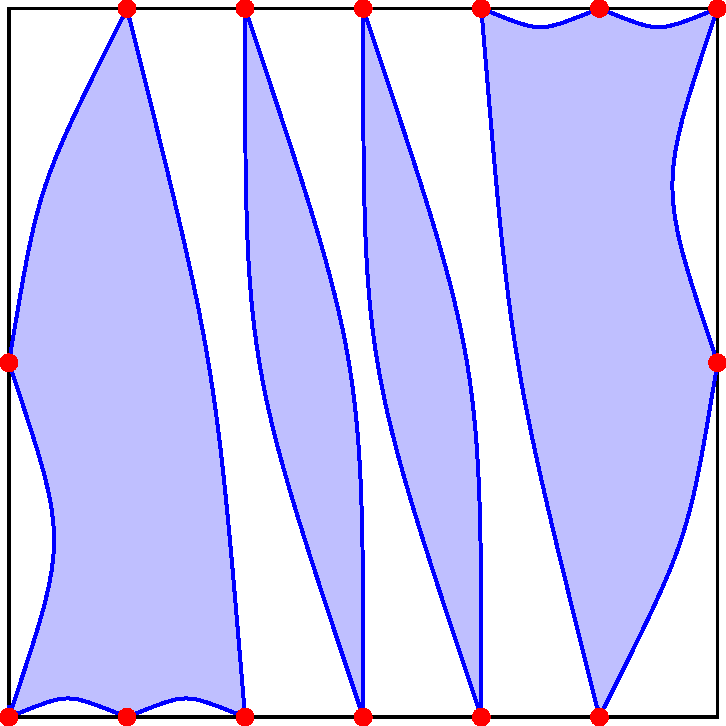
\includegraphics[width=4.1cm]{constr2clear.pdf}};};
\foreach \a in 
    {(7,0), (7,4), (7,8), (7,12)}
    {\draw[line width=0.5mm, black!50] \a rectangle ++(4,4);
    \fill 
        \a++(0.8,2) circle (0.25)
        \a++(1.6,2) circle (0.25)
        \a++(2.4,2) circle (0.25)
        \a++(3.2,2) circle (0.25);
        };
\foreach \a in 
    {(7,0), (7,4), (7,8)}
    {\draw[line width=0.7mm]
        \a++(0.8,2) -- ++(0,4)
        \a++(1.6,2) -- ++(-0.8,4)
        \a++(2.4,2) -- ++(-0.8,4)
        \a++(3.2,2) -- ++(-0.8,4)
        \a++(3.2,2) -- ++(0,4);
    };
\end{tikzpicture}
\end{document}